\documentclass[12pt]{elsart}
\usepackage{amsmath}
\usepackage{amssymb}
\usepackage{color}
\usepackage{graphicx}
\newcommand{\field}[1]{\mathbb{#1}}

\usepackage{program}
\usepackage[makeroom]{cancel}

\usepackage{algorithm}
\usepackage{algpseudocode}

%%%%%%%%%%%%%%%%%%%%%%%%%%%%%%%%%%%%%%%%%Space to make more readable!
%\vspace{10 mm}
%%%%%%%%%%%%%%%%%%%%%%%%%%%%%%%%%%%%%%%%%Take out later!

%\usepackage[letterpaper,top=0.75in, bottom=0.75in, left=1in, right=1in]{geometry}

\begin{document}

\pagestyle{empty}

\begin{center}
\Large  CS5463 Fundamentals of Software  - Fall 2020 \\
\large {\bf Assignment 1: Function Runtimes Table}\\
\normalsize Due 9/10/20 by 11:59pm
\end{center}

{\bf Completing the Program (15 points)}

This program prints a table of runtimes (these are displayed in seconds) for given functions on arrays.  The program tests different array sizes to establish a relationship between input size and runtime.  It tests each array size multiple times and then takes an average of the times.  Here are example calls to the timing functions:

\begin{quote}
\small
\begin{verbatim}
int[] sizes1= { 1000, 2000, 4000, 8000, 16000};

fRT = timeAlgorithm("Insertion Sort", 10, 5, sizes1, "insertionSortInitial" );
printRuntimeTable(fRT);

fRT = timeAlgorithm("quicksort", 10, 5, sizes1, "quickSortOptInitial" );
printRuntimeTable(fRT);
\end{verbatim}
\end{quote}


This results in following table:

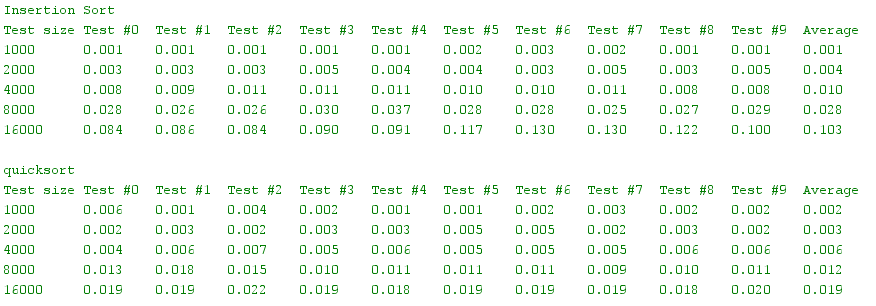
\includegraphics[width=16cm]{ExampleTable}

Note your runtimes may vary since the test data is randomly generated.

The runtimes are stored in a functionRuntimes class.  You are completing a program to create and fill data in this class, print the data of this class.  

You are given a partial implementation in the files ``MysteryRuntime.java", ``functionRuntimes.java", and ``ArrayAlgs.java".  The portions of code that you need to write have been marked with the text ``TODO''.

{\bf Using the Program (5 points)}

After you have the program completed, you should use it to help determine the asymptotic runtimes of the three mystery functions (i.e., mysteryRuntime1, mysteryRuntime2, mysteryRuntime3).   

Be sure to also examine the code of the mystery functions to confirm your estimations.

Fill in the following table with your runtimes:

\begin{quote}
\small
\begin{verbatim}
/*
Give your asymptotic estimates for the runtimes of the following 3 functions:

mysteryRuntime1:  O(   )
mysteryRuntime2:  O(   )
mysteryRuntime3:  O(   )
*/
\end{verbatim}
\end{quote}

{\bf 1. Longest Sorted Subarray (4 points)}

Consider the following problem:

{\bf Input:} An array $A[1 \ldots n]$ of integers \\
{\bf Output:} The largest integer $m$ such that the array $A[1 \ldots n]$ has subarray of length $m$ which is in sorted order (i.e, increasing order).

The following pseudocode finds the length of the longest of the given array $A[1\ldots n]$ by considering all possible subarrays:

\begin{algorithm}
\caption{longestSubArray( int $A[1\ldots n]$ )}
 \begin{algorithmic}[1]
 %
 \State $k = n$;
 \While{( $true$ )}
 \State //(I) The longest increasing subarray of $A$ has length $\leq k$
  \State $low = 1$
 \State $high = k$

   \While{( $high\leq n$ )} 
       \If{( $isIncreasing(A[low \ldots high])$ )} 
\State return $k$;
\EndIf
       \State $low++$
       \State $high++$
    \EndWhile
    \State $k--$;
  \EndWhile
\end{algorithmic}
\end{algorithm}

The following code checks if an array is increasing (i.e., each number is smaller than the next in the array).

\begin{algorithm}
\caption{isIncreasing( int $C[a\ldots b]$ )}
 \begin{algorithmic}[1]
 %
 \State $i = a$;
 \While{$i<b$}
 \If{( $C[i]\geq C[i+1]$ )} 
\State return $false$;
\EndIf
   \State $i++$;
 \EndWhile
\State return $true$;
\end{algorithmic}
\end{algorithm}

{\bf Example:}  longestSubArray( $[ 2, 4, 3, 8, 5, 6, 7, 9, 0, 1 ]$ ) returns 4 \\
{\bf Justification:} $[ \cancel{2, 4, 3, 8}, 5, 6, 7, 9, \cancel{0, 1} ] = [ 5, 6, 7, 9 ]$ which is a longest increasing subarray of the original array.

\begin{enumerate}
   \item (2 points) Consider running longestSubArray on the array:\\ 
   
   \begin{quote}
   $[119,100,112,114,125,113,110,129,130,140,142,115,120]$\\
   \end{quote}
   
   What does longestSubArray return and what is the longest sorted subarray of $A$?
   \item (1 point) Give the best-case runtime of longestSubArray in asymptotic (i.e., $O$) notation as well as a description of an array which would cause this behavior.  
   \item (1 point) Give the worst-case runtime of longestSubArray in asymptotic (i.e., $O$) notation as well as a description of an array which would cause this behavior.  
   \item (0 points) Is this an efficient algorithm for finding the longest sorted subarray?  Can you find a better algorithm for computing this?
\end{enumerate}


{\bf 2. Asymptotic Notation (4 points)}

Show the following using the definitions of $O$, $\Omega$, and $\Theta$.

\begin{enumerate}
   \item (2 points) $2n^3+n^2+4\in \Theta(n^3)$
   \item (2 points) $3n^4-9n^2+4n\in \Theta(n^4)$\\  ({\bf Hint:} careful with the negative number)
\end{enumerate}

{\bf Deliverables:}

Your solution should be submitted as ``MysteryRuntime.java" as well as a .pdf file with your answers to written part of the assignment.  Be sure to fill in the table of runtimes described above:

Upload this file to Blackboard under Assignment 1.  {\bf Do not zip your file}. 

To receive full credit, your code must compile and execute. You should use valgrind to
ensure that you do not have any memory leaks.

{\bf Remember:  

The program you submit should be the work of only you. Cheating will be reported to SCCS. Both the copier and copiee will be held responsible.}


\end{document}